\subsection{Ring-Imaging Cherenkov (RICH)}

One of the six CLAS12 Forward Carriage sectors has been equipped with a Ring Imaging Cherenkov detector \cite{rich-nim}.

\subsubsection{Geometry}
The RICH mirror geometry is implemented through both of the native GEMC geometry API and imports from the engineering model STEP files.
The spherical mirrors are made through Geant4 boolean intersections of spheres and planes.
Since the array of 391 PMTs is inside the CLAS12 acceptance, particular care went into implementing in the
simulation the details of the PMT hardware and materials: the PMTs are Geant4 aluminum boxes containing the electronics components
(including the adapter, ASIC and FPGA boards), the window, the photocathodes.
Each PMTs contain 64 pixel. The identification of the pixel is done in the process identification routine.
The aerogel are Geant4 boxes.
The RICH box, mirror support structure, and additional support hardware are imported directly from the engineering CAD models.
\F{richGeometry} shows details of the geometry implementation.

\begin{figure}
	\centering
	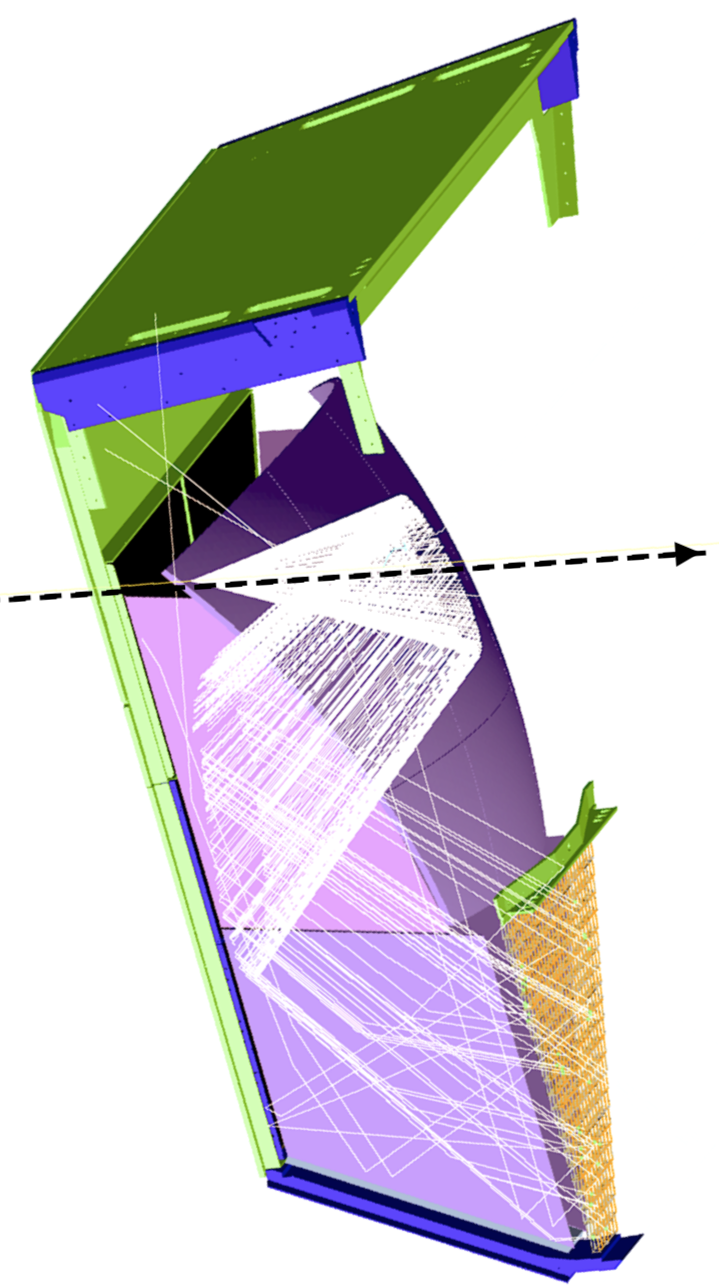
\includegraphics[width=0.99\columnwidth, keepaspectratio]{img/richGeometry.png}
	\caption{The implementation of the RICH geometry. Beam is incident from the left. A 4 GeV kaon produces a Cherenkov light cone.
			 Part of the cone reflects onto the spherical mirror and into the PMT array. The remaining photons go through the aerogel tiles
			 and bounce off the planar mirror onto the PMT array. All inefficiencies are taken into account by using the aerogel refractive index
			 and its transparency. }
	\label{fig:richGeometry}
\end{figure}

The refractive index of the aerogel and its transparency is included in the material optical properties and taken
into account during the Geant4 transportation of the photons.
Similarly for the reflectivity of the mirrors. The quantum efficiency associated with the PMT photocathodes is taken into account in the digitization routine.

\subsubsection{Process ID}
At each Geant4 step, the local coordinates in the PMT volume are used to calculate the pixel number within that PMT.

\subsubsection{Digitization}

Photons that impinge on the PMT faces are processed with the digitization routine.
Each photon collected is input to the quantum efficiency algorithm at its wavelength to decide if it is detected.
The ADC energy is calculated and smeared using the single photo-electron peak position and width from the calibration database.
The time average of all the photons is saved in the output.
The digitized output bank variables are summarized in Table \ref{tab:richBank}.

\begin{table}[h]
	\begin{center}
		\begin{tabular}{| c | c | c |}
			\hline \hline
			Variable & Description                                         \\
			\hline
             sector  &                                     CLAS12 sector   \\
                pmt  &                                        PMT number   \\
              pixel  &                       pixel number within the PMT   \\
                ADC  &                                               ADC   \\
               time  &                           average time of the hit   \\
               nphe  &                  number of photoelectrons arrived   \\
              npheD  &                 number of photoelectrons detected   \\
               hitn  &                                        hit number   \\
			\hline \hline
		\end{tabular}
	\end{center}
	\caption{The digitized RICH bank.}\label{tab:richBank}
\end{table}

The time window  of the RICH is set to 5 ns: all Geant4 steps within the same PMT pixel and time window are collected in one hit.
